\documentclass[a4paper,10pt]{article}
%\usepackage[utf8x]{inputenc}

\usepackage{graphicx}
\usepackage{float}
\usepackage{caption}
\usepackage{subcaption}
\usepackage{amsmath}


%opening
\title{Assignment 4: Optical Flow and Structure from Motion}
\author{Robrecht Jurriaans (5887380), Taco Cohen (6394590)}

\begin{document}

\maketitle

\section{Optical Flow}
We have implemented Lucas-Kanade optical flow for a single scale on both synthetic images and on a sequence of a model house. For the synthetic images, optical flow was computed on a grid of non-overlapping $15x15$ windows, whilst a set of points was tracked over the model house sequence. We created two separate functions for this: \verb|LucasKanade.m| for the non-overlapping windows and \verb|LK_M.m| for the tracking. 

\begin{figure}[h!tb]

        \centering
        \begin{subfigure}{0.475\textwidth}
                \centering
                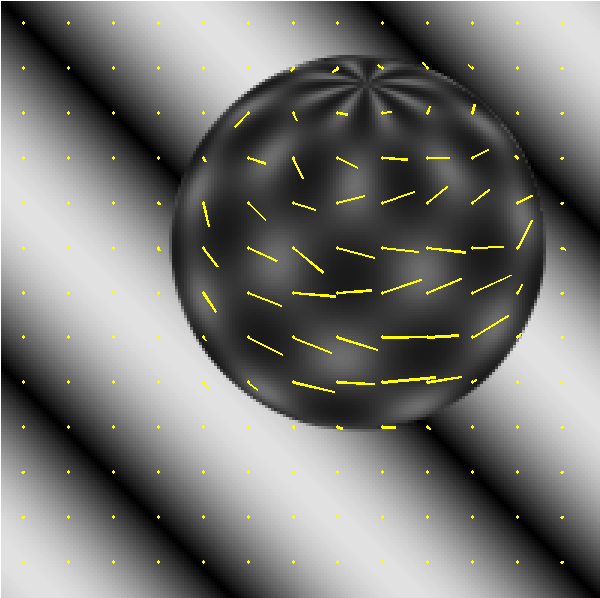
\includegraphics[width=\textwidth]{sphere}
                \caption{Optical flow for the sphere images}
        \end{subfigure}
        ~
        \begin{subfigure}{0.475\textwidth}
                \centering
                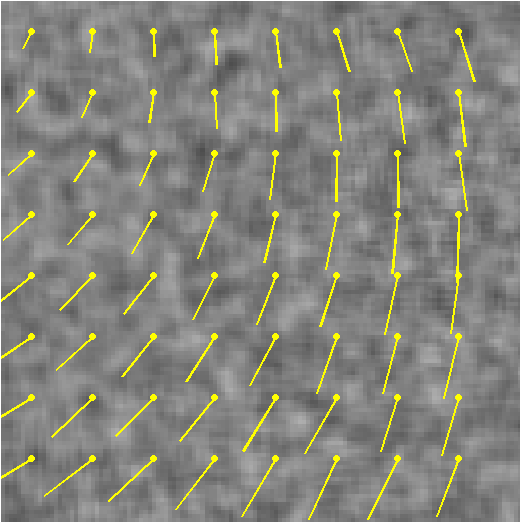
\includegraphics[width=\textwidth]{synth}
                \caption{Optical flow for the synth images}
        \end{subfigure}
\caption{Optical flow for non overlapping $15x15$ windows, circle denotes origin of optical flow vector}
\label{fig:opflow}      
\end{figure}

\subsection{Sphere and Synthetic Images}
In figure \ref{fig:opflow} the resultant optical flow vectors can be seen for both the \emph{sphere} images as the \emph{synth} images. The sphere is turning to the right, which can be seen in the optical flow vectors on the sphere. Some of the flow vectors seem to be a bit off, but this is mainly because the windows were not centred at good features which would improve results. The synthetic image rotates slightly, and this result can be seen on the right with optical flow vectors with a relatively small magnitude.



\subsection{Optical flow on the model house sequence}
The model house sequence consist of 101 frames with 215 given points which can be tracked. In figure \ref{fig:modelhouse} the 100th frame can be seen with the ground truth and the corresponding points as tracked by the algorithm. The final sum of squared errors is $337.3183$ and the median squared error is $17.3528$. The main contributor to the error are points which drift into ``flat'' regions in which no motion can be observed causing the points to further drift away from the ground truth. Another contributor is the \emph{jpg} compression of the sequence, causing noise in the data which result in less precise optical flow vectors.

\begin{figure}[h!tb]
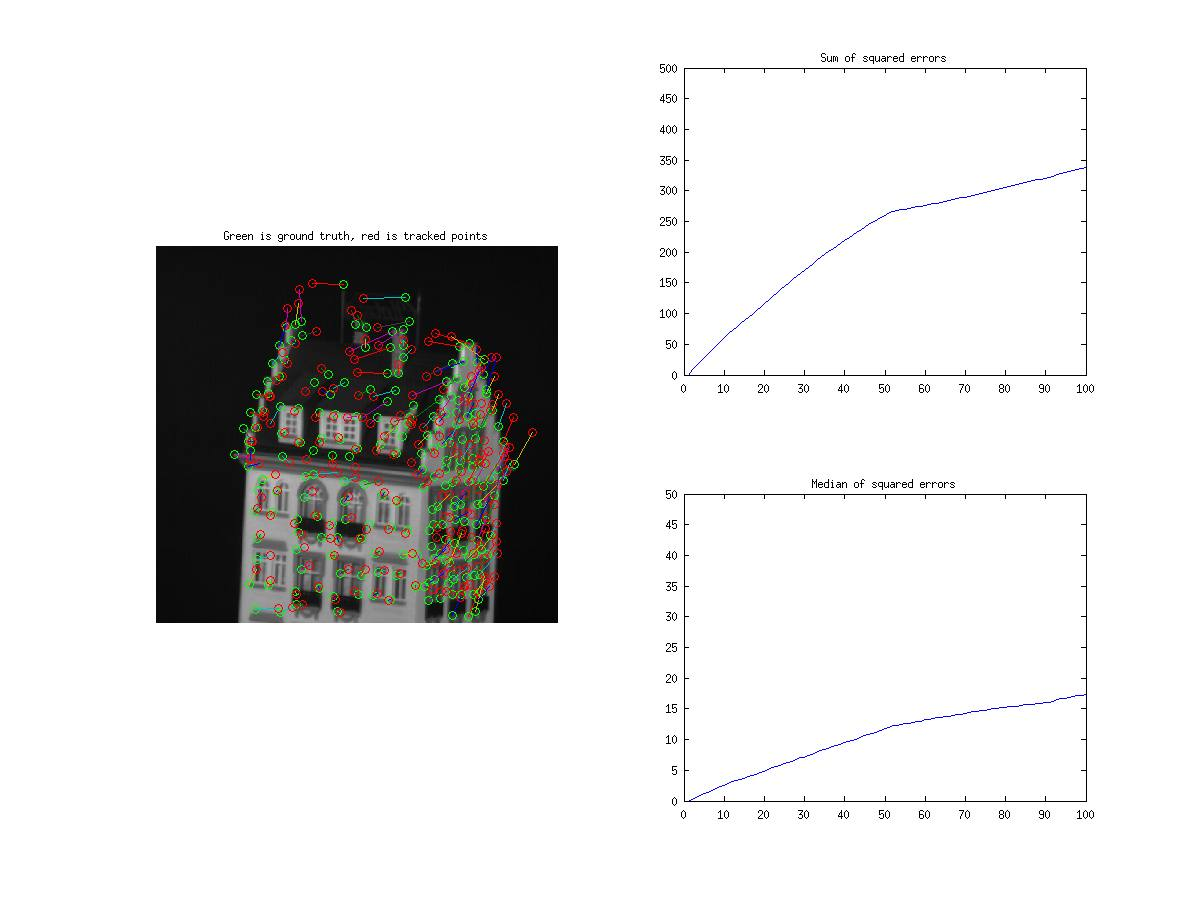
\includegraphics[width=1\textwidth]{frame00000100}
\caption{Frame 100 from the model house sequence, green circles represent ground truth, red circles are the points tracked over all 100 frames, lines connect corresponding points, the graphs represent the sum of squared errors and the median of squared errors over the sequence }
\label{fig:modelhouse}
\end{figure}

A movie was created of the output frames: \verb|opflow.avi| in which this effect can be clearly seen. This is especially the case for the points on the left of the house which drift into the dark background.

\clearpage

\section{Structure from Motion}



\end{document}
